\documentclass{standalone}
\usepackage{standalone}

\begin{document}
\section{Artificial Neural Network}

Inspired by the functionality of neural network, researchers tried make something similar and that is artificial neural network (ANN). The neurons takes some information as input via Dendrites, processes it and then sends to next neuron until it reaches destination. Similar to this ANN is shown in figure 3.4,
\\
\begin{figure}[h]
				\centering
				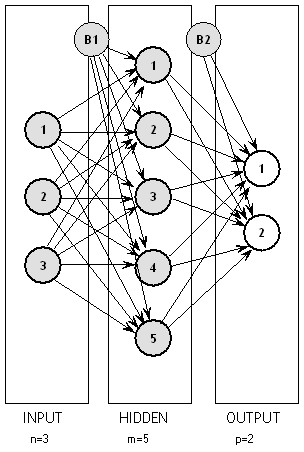
\includegraphics[scale=0.9]{./img/nn}
				\caption{Basic Artificial Neural Network} \label{fig:mapComp}
\end{figure}
\\
Ann consists of few parts, 
\begin{itemize}
  \item Nodes which are shown as input, hidden and output layer.
	\item Edges which contains weights.
	\item Activation function. It defines whether a neuron will fire or not with a certain limitation.
  \item Bias input node that helps to find the solution faster and in other field as well. Except output layer, all layers contains bias node.
\end{itemize}

As shown in the figure, the input node is connected with all node of hidden layer except bias. The hidden layers are connected with all output nodes. The weights are initialized with random numbers. 
ANN works in two phases: forward phase and backward phase. The Input node takes the inputs, processes it by multiplying the weight corresponded to the edge and sends it to next layer. Similarly hidden layer takes the input that was given, processes it using an activation function, then similarly the output is multiplied with the corresponding weight and sends it to output layer. The output layer takes the inputs, processes it and gives a corresponding output. This is called forward phase. In backward phase the weights are updated according to the output. In forward phase the following equation is used as activation function: \\

\begin{center}
	\makebox g(x) = $ \frac {1}{1+e^{-\beta}x} $\\
\end{center}


Here, $ \beta $  is a random number.\\
The calculations for in each neuron k in hidden layer is given below: \\
 
\begin{center}
	\makebox h\textsubscript{k}= $\sum_{n=0}^{L} x\textsubscript{i}v\textsubscript{ik}$
\end{center}
\begin{center}
	\makebox a\textsubscript{k} = g(h\textsubscript{k})= $ \frac {1}{1+exp(-\beta h\textsubscript{k})}$
\end{center}
Here, L is the number of input nodes. The calculations for in each neuron j in output layer is given below:\\
\begin{center}
	\makebox  h\textsubscript{j}= $\sum_{j} a\textsubscript{k}w\textsubscript{jk}$
\end{center}
\begin{center}
	\makebox y\textsubscript{j} = g(h\textsubscript{j})= $ \frac {1}{1+exp(-\beta h\textsubscript{j})}$
\end{center}
Here, N is the number of nodes in hidden layers.\\
The following equations are used for updating the weights in output layer:\\
\begin{center}
	\makebox  \delta\textsubscript{o}(j) = (y\textsubscript{j} - t\textsubscript{j}) y\textsubscript{j} (1-y\textsubscript{j})  \\
\end{center}
\begin{center}
	%\makebox  \delta\textsubscript{o}(k) = (y\textsubscript{k} - t\textsubscript{k}) y\textsubscript{k} (1-y\textsubscript{k})  \\
	\makebox  w\textsubscript{jk} \Leftarrow w\textsubscript{jk} - \eta\delta\textsubscript{o}(j)a\textsubscript{k} \\
\end{center}
Here $\eta$ is the learning rate. The following equations are used for updating the weights in hidden layer:\\
\begin{center}
	\makebox  {$\delta$\textsubscript{h}(k) =  a\textsubscript{k}(1-a\textsubscript{k})\sum_{j=1}^{N} w\textsubscript{jk}$\delta$\textsubscript{o}(j)}
\end{center}
\\
\begin{center}
	\makebox  v\textsubscript{ik} =  v\textsubscript{ik} - $\eta\delta\textsubscript{h}(k)x\textsubscript{i}  $\\
\end{center}
ANN works well with large data set. So, if the data set is too small then it will not perform well. The output often depends on number of iteration and number of node in hidden layer. \\


\end{document}